\section{Evaluation}
In this section, we evaluate the real-time performance, visual consistency, and realism of our system, highlighting the contributions of our technical innovations with ablation studies. Unless stated otherwise, the experimental setup is as follows: The simulation uses a grid resolution of \(64^3\) with 8 particles per grid cell at initialization. Each frame performs 5 simulation substeps, employing a neo-Hookean elasticity model (Young's modulus \(E=10^6 Pa\), Poisson's ratio \(\nu=0.3\))  combined with a von Mises plasticity model (yield stress \(\sigma_y=10^5 Pa\)). For rendering, the density field is sampled at \(128^3\), with mesh reconstruction via the Marching Cubes algorithm and 5 iterations of Laplacian smoothing to improve surface quality. To ensure consistent comparisons, we recorded a specific hand trajectory for each example and applied it across all tests with varying parameters.

\paragraph{Real-Time Performance}
To evaluate the real-time performance of VR-Doh, we conducted an experiment involving a simple scenario where a sphere is compressed between two hands (as shown in \autoref{fig:Boundary_Projection}, bottom row). To analyze performance scalability, we varied the simulation grid resolution, the number of substeps per frame, and the number of particles per grid cell, while keeping other parameters constant. The overall FPS under these conditions is summarized in \autoref{fig:performance}. The results demonstrate that VR-Doh can maintain real-time performance, achieving interactive frame rates even with higher computational demands, such as a \(100^3\) simulation grid resolution, 30 substeps per frame, and 12 particles per cell.

\begin{figure*}[ht]
    \centering
        \includegraphics[width=0.8\linewidth]{img/performance.pdf}
        
    \captionof{figure}{\textbf{Real-Time Performance Evaluation.} FPS of VR-Doh with varying simulation grid resolution, substeps per frame, and MPM particles per cell in a sphere compression scenario (\autoref{fig:Boundary_Projection}, bottom). Results demonstrate VR-Doh's ability to maintain real-time performance under high computational demands.}
    \label{fig:performance}
\end{figure*}
\paragraph{Convergence Under Spatial Refinement}
To validate the consistency of our simulation, we conducted an experiment where a hand trajectory presses into a sphere to create a hole and then squeezes it from both sides. The simulation was tested with varying grid resolutions while keeping the number of particles per cell constant. As shown in \autoref{fig:reso}, the deformations converge once the grid resolution exceeds \(48^3\), indicating that our simulation achieves consistent and accurate results without requiring excessively high resolutions.

\begin{figure*}[htbp]
    \centering
        \includegraphics[width=0.65\linewidth]{img/reso_new.pdf}
        
    \captionof{figure}{\textbf{Convergence under Spatial Refinement.} Sphere deformations under identical hand imprints and squeezing converge at resolutions above $48^3$, ensuring accuracy without excessive computational cost.}
    \label{fig:reso}
\end{figure*}


% \subsection{Ablation Studies}
% We conducted several ablation studies to demonstrate the necessity and efficacy of our technical contributions.


%我们记录了一段手的轨迹,并在不同边界条件下,作用在相同物体上。图?分别展示了仅使用MPM标准边界条件,仅使用Particle-Level Boundary Projection,以及两者都采用的效果。第一行中,我们尝试用手在一个球上留下一个印记,用于展示细节调整能力。第二行中,我们用双手挤压一个较小的球,用于展示整体调整能力。可以看到,加入Particle-Level Boundary Projection后,留下的印记清晰了很多,提高了细节调整的能力。而第二行的结果表明,仅使用Particle-Level Boundary Projection无法做到volume conservation。这是因为这一阶段的形变信息无法被记录在grid_level的形变矩阵中。因此,将这两者结合能实现both在整体上的真实形变以及细节部分的调整。
\begin{figure}[ht]
    \centering
    \includegraphics[width=0.9\linewidth]{img/Adjust_Particle.pdf}
        
    \captionof{figure}{ {\textbf{Particle-Level Collision Handling.} Comparison of MPM boundary conditions with and without particle-level collision handling on a hand imprint (top) and a sphere compression (bottom) example. Combining both methods (right) achieves realistic deformations with enhanced detail while avoiding volume loss.}}
    \label{fig:Boundary_Projection}
\end{figure}
\paragraph{Particle-Level Collision Handling}
In \autoref{fig:Boundary_Projection}, we compare the traditional MPM boundary condition with and without our particle-level collision handling using a hand imprint (top row) and a sphere compression (bottom row) example. As shown in the figure, applying particle-level collision handling produces significantly clearer imprints, enhancing the ability to adjust finer details. However, the results in the second row demonstrate that using only particle-level collision handling can lead to severe volume loss, as the particle projection step does not account for elastoplasticity forces. By combining both methods, our approach achieves realistic overall deformations while enabling precise adjustments for detailed modeling.



\paragraph{Localized Simulation}
\begin{table}[H]
\centering
\caption{ \textbf{Localized Simulation.} Comparison of FPS with and without localized simulation in large 3D Gaussian Splatting scenes, showing an average frame rate improvement of $\mathbf{3.3\times}$ with localized simulation enabled.}
\label{tab:local}

\begin{tabular}{>{\centering\arraybackslash}m{1cm}|>{\centering\arraybackslash}m{1.5cm}|>{\centering\arraybackslash}m{2.4cm}|>{\centering\arraybackslash}m{2.2cm}}
\toprule
\textbf{Scene} & \textbf{Splats count} & \textbf{FPS w/o localized  sim.} & \textbf{FPS w localized sim.} \\
\hline
Garden & 660K & 12.2 & \textbf{39.8} \\
\hline
Bicycle & 480K & 13.1 & \textbf{43.5} \\
\hline
Room & 382K & 13.6 & \textbf{44.5} \\
\bottomrule
\end{tabular}
\end{table}

We evaluated VR-Doh's performance with and without localized simulation across several typical 3D GS scenes, including Garden, Bicycle, and Room, each containing several hundred thousand Gaussians. During the tests, users navigated through each scene and interacted with primary objects using hand gestures, introducing deformations. As shown in \autoref{tab:local}, enabling localized simulation resulted in an average frame rate improvement of $3.3\times$, demonstrating its significant impact on performance.

\paragraph{Uniform Gaussian Volume Regularizer}
We evaluated the effectiveness of our Uniform Gaussian Volume Regularization by simulating a textured sand cube represented with 3D Gaussians as it was dropped onto the ground under gravity, resulting in significant deformations. \autoref{fig:Regularizer} compares the original model (left) with the deformed results using (middle) and without (right) the proposed volume regularization loss, both trained for 30,000 iterations using Adam \cite{Kingma2014AdamAM}. Without the loss, the exposed interior reveals noticeable blurry artifacts caused by uneven Gaussian volumes. In contrast, applying the regularization maintains consistent Gaussian volumes, preserving sharp details and achieving high visual fidelity even under extreme deformation. 
\begin{figure}[ht]
    \centering
        \includegraphics[width=\linewidth]{img/Big_Gaussians.pdf}
        
    \captionof{figure}{  \textbf{Uniform Gaussian Volume Regularizer.} Comparison of a sand cube dropped under gravity shows that applying the regularization (middle) preserves sharp details and avoids blurry artifacts in the interior (right), ensuring high visual fidelity during large deformations.}
    \label{fig:Regularizer}
\end{figure}
\paragraph{Decoupled Appearance and Physical Representations}
We evaluated the performance of our method under different sampling ratios between MPM particles and Gaussian kernels in a simulation where a wolf sits on the ground under gravity. Here, we maintain the MPM particle per cell, so the simulation grid resolution decreases as we downsample MPM particles. \autoref{fig:Improved_gaussian} illustrates the original (left) and deformed (right) configurations and the FPS achieved with varying sampling ratios. The results show that as the sampling ratio decreases—fewer MPM particles driving the 3D Gaussians—the wolf's volume slightly increases while maintaining high visual fidelity and preserving detailed features. This behavior is expected, as lower resolutions in MPM typically exhibit stiffer deformation due to discretization errors. Notably, by reducing MPM particles to approximately $30\%$ of the Gaussian kernels, the FPS nearly doubles, demonstrating the effectiveness of our approach to decouple appearance and physical representations, achieving significant performance gains without sacrificing visual quality.
\begin{figure}[htbp]
    \centering
    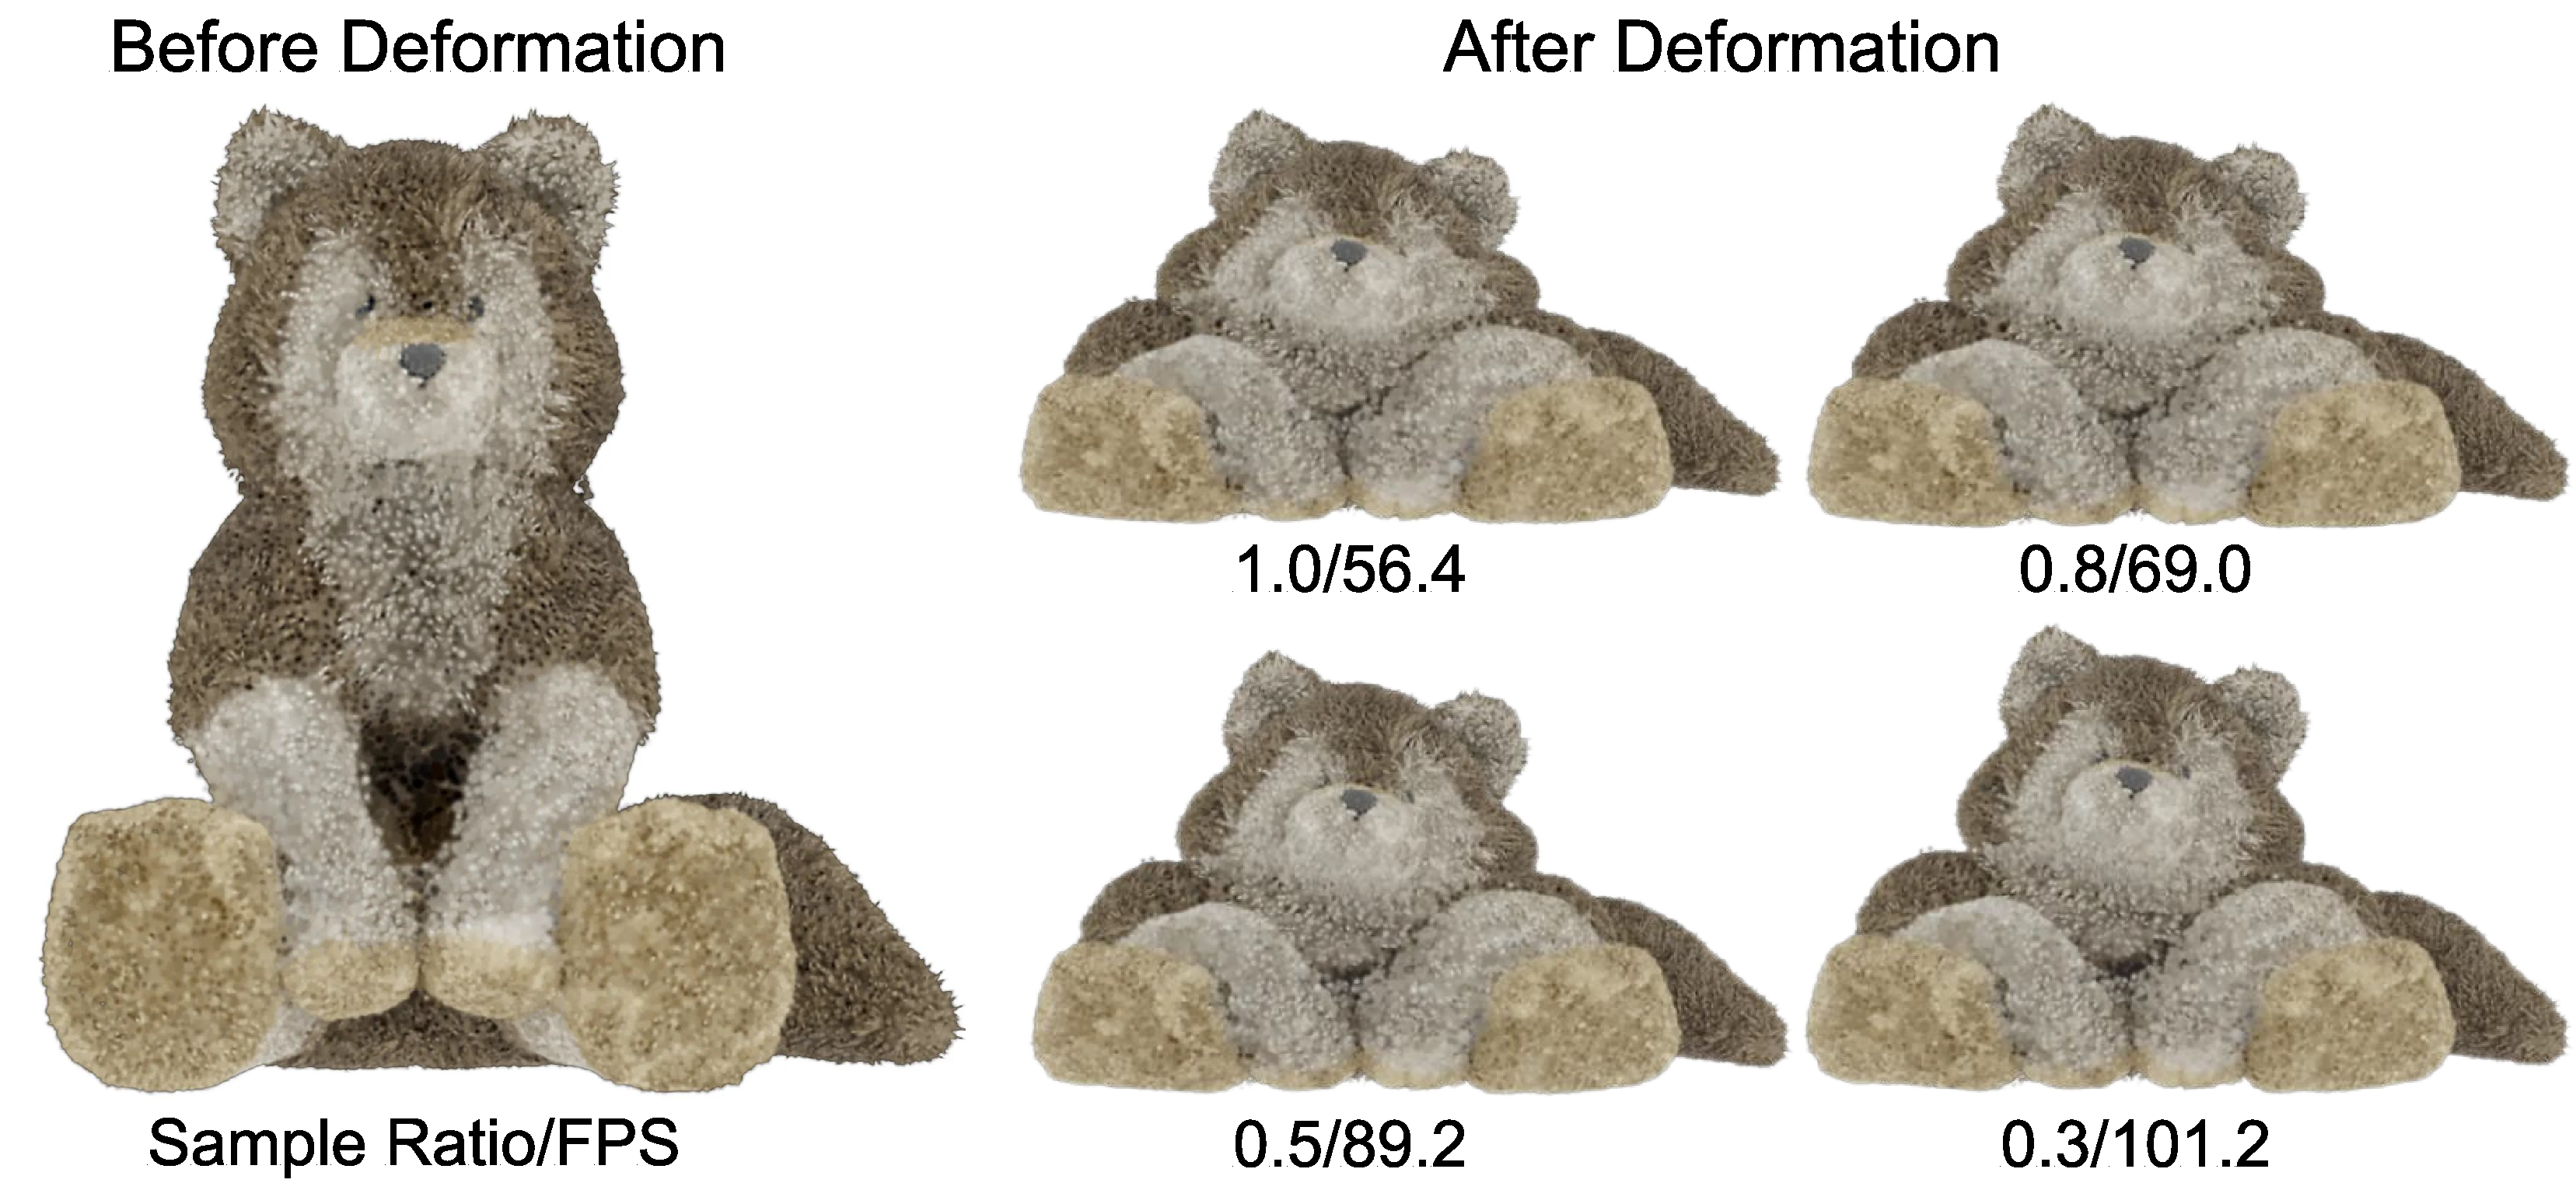
\includegraphics[width=1.0\linewidth]{img/Improved_Gaussian.pdf}
    \caption{ {\textbf{Decoupled Appearance and Physical Representations.} This example of a wolf sitting under gravity demonstrates that reducing the number of MPM particles driving the 3D Gaussians slightly increases the wolf's volume but maintains high visual fidelity while significantly improving FPS, showcasing the effectiveness of our approach. }}
    \label{fig:Improved_gaussian}
\end{figure}


